\documentclass{beamer}
\usetheme{Madrid}
\usecolortheme{beaver}
\usepackage{amsmath}
\usepackage{verbatim}

\title{Coordinate Geometry}
\subtitle{Using Matrix Analysis}
\author{Haveesh Singirikonda\\Prashanth Babu}
\institute{IIT Hyderabad}
\date{\today}

\begin{document}

\begin{frame}
\titlepage
\end{frame}
\begin{comment}
\section{Introduction}

\begin{frame}

\frametitle{Matrix Analysis in Coordinate Geometry}
Coordinate Geometry gets much more simpler and easier when Matrices are used to represent points and equations. \\
Matrix transformations can be used in most scenarios to compute distances and to find the equations of lines and conics.

\end{frame}
\end{comment}
\section{The Problem}
\subsection{Problem Statement}

\begin{frame}
\frametitle{Question}
One of the diameters of the circle, given by $$ x^2 + y^2 -4x+6y = 12$$ 
is a chord of the circle S whose centre is at (-3,2).
Find the radius of S.

\end{frame}

\begin{frame}
\frametitle{Question in MATRIX Form}
One of the diameters of the circle, given by $$ \mathbf{X^TX} + 2\left[
\begin{matrix}
-2 & 3 
\end{matrix}
\right]\mathbf{X} = 12 $$ is a chord of the circle S whose centre is at 
$$
\left[
\begin{matrix} 
-3 \\
 2
\end{matrix}
\right] $$ Find the radius of S.
\end{frame}

\subsection{Figure}
\begin{frame}
\frametitle{Figure}
\includegraphics[scale=0.5]{/home/haveesh/Pictures/circle.png}
\end{frame}

\section{Solution}


\begin{frame}
\frametitle{Solution}
Points on a circle with centre $ \mathbf{C} $ and radius $\mathbf{R}$ would follow $$ (\mathbf{X} - \mathbf{C})^T(\mathbf{X} - \mathbf{C}) = R^2 $$

Simplifying it :
$$ \mathbf{X^TX} + \mathbf{C^TC} - \mathbf{C^TX} - \mathbf{X^TC} = R^2 $$

In this case :
$$ \mathbf{C^TX} = \mathbf{X^TC} $$ 
As \textbf{X} and \textbf{C} are one dimensional arrays.
\end{frame}

\begin{frame}
\frametitle{Solution}
So the equation of a circle centered at \textbf{C} and of radius \textbf{R} is
$$ \mathbf{X^TX} - 2\mathbf{C^TX} = R^2 - \mathbf{C^TC} $$
Now comparing it with 
$$ \mathbf{X^TX} + 2\left[
\begin{matrix}
-2 & 3 
\end{matrix}
\right]\mathbf{X} = 12 $$
We get
$$ \mathbf{C} = \left(\begin{matrix}
2 \\
-3
\end{matrix} \right)
$$
$$ R^2 - \mathbf{C^TC} = 12 $$
$$ R = 5 $$ 

\end{frame}

\begin{frame}
\frametitle{Solution} 

Given that chord of circle \textbf{S} is the diameter of the circle centered at \textbf{C}

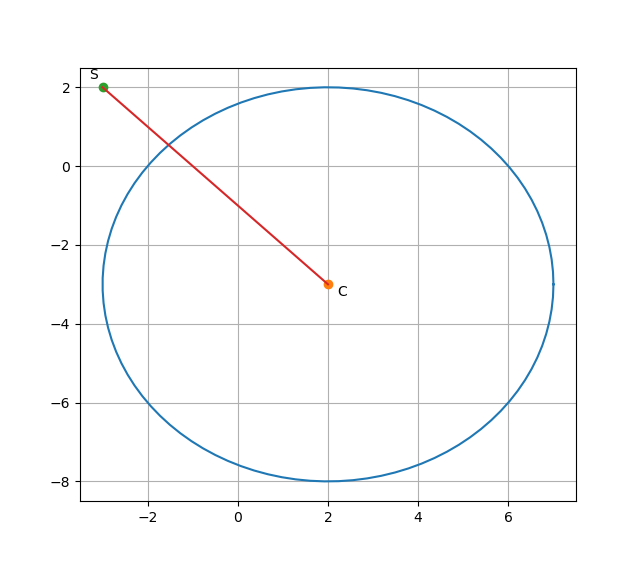
\includegraphics[scale=0.5]{/home/haveesh/Pictures/Figure_2.png}
\end{frame}

\begin{frame}
\frametitle{Solution}
\textbf{CS} would be perpendicular to the chord of \textbf{S} i.e, is perpendicular to a diameter of \textbf{C} \\
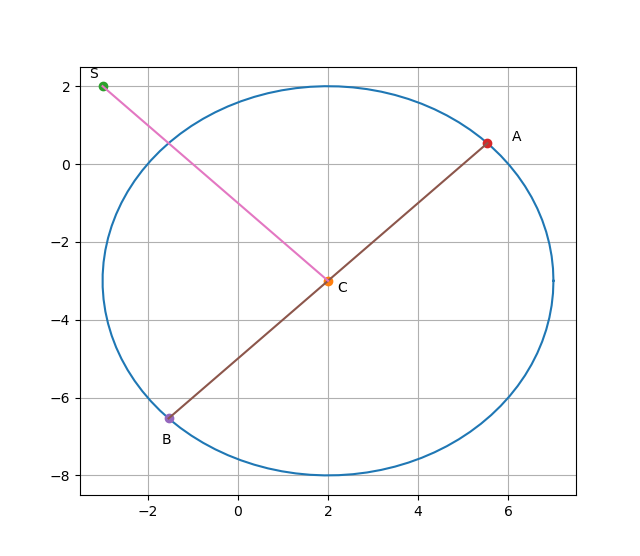
\includegraphics[scale=0.5]{/home/haveesh/Pictures/Figure_3.png}
\end{frame}

\begin{frame}
\frametitle{Solution}
To find the points \textbf{A} and \textbf{B}, we find the points of intersection of the diameter perpendicular to \textbf{SC} and the circle. 

If \textbf{D} is the direction vector of \textbf{SC}
$$ D = S - C$$
$$ D = \left( \begin{matrix}
-5 \\
5
\end{matrix} \right) $$
\end{frame}

\begin{frame}
\frametitle{Solution}
For the line \textbf{AB}, it's normal $\mathbf{{N}}$ is parallel to $\mathbf{SC} $ \\
So we can take 
$$ \mathbf{N} = \left(\begin{matrix}
1 \\
-1
\end{matrix} \right) $$ 
Equation of \textbf{AB} is 
$$ \mathbf{N^TX} = p $$
As the centre of circle \textbf{C} passes through this line, 
$$ \mathbf{N^TC} = p$$
$$ p = 5 $$ 
Equation of \textbf{AB}
$$ \left(\begin{matrix}
1 & -1
\end{matrix} \right)
\mathbf{X} = 5 $$
\end{frame}

\begin{frame}
\frametitle{Solution}
Equation of circle in parametric form is
$$ \mathbf{X} = \mathbf{C} + R\mathbf{{\Theta}} $$
Where
$$ \mathbf{\Theta} = \left(\begin{matrix}
cos\theta \\
sin\theta
\end{matrix} \right) $$
$$ \mathbf{C} = \left(\begin{matrix}
2 \\
-3
\end{matrix} \right) $$
Substituting this in the line equation would give us the value of $\theta$ at \textbf{A} and \textbf{B}
\end{frame}

\begin{frame}
\frametitle{Solution}
After substitution we get 
$$ \mathbf{N^T}\left[\mathbf{C}+R\mathbf{{\Theta}}\right]= p $$ 
$$ \mathbf{N^T\Theta} = \frac{p-\mathbf{N^TC}}{R}  $$
We get
$$ cos\theta = sin\theta $$
In the range $\theta\in\left[0,2\pi\right]$ 
$$ \theta = \frac{\pi}{4},\frac{5\pi}{4} $$
$$ \mathbf{A} = \left(\begin{matrix}
2+\frac{5}{\sqrt{2}} \\
-3+\frac{5}{\sqrt{2}}
\end{matrix} \right) $$
$$ \mathbf{B} = \left(\begin{matrix}
2-\frac{5}{\sqrt{2}} \\
-3-\frac{5}{\sqrt{2}}
\end{matrix} \right) $$
\end{frame}

\begin{frame}
\frametitle{Solution}
$\Delta\mathbf{BCS}$ and $\Delta\mathbf{ACS}$ are right angled triangles.
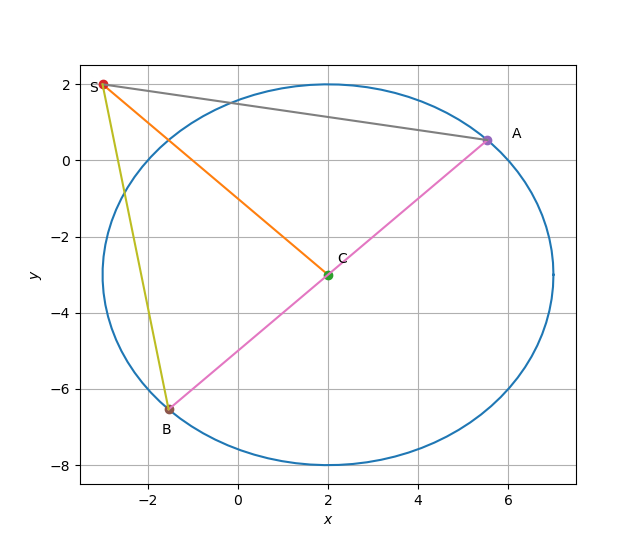
\includegraphics[scale=0.53]{/home/haveesh/Pictures/Figure_4.png}
\end{frame}

\begin{comment}
	\begin{frame}
	\frametitle{Solution}
	The distance \textbf{SC} is 
	$$ d^2 = \left( \mathbf{S}-\mathbf{C} \right)^T\left( \mathbf{S}-\mathbf{C} \right) $$
	
	Where \textbf{S} and \textbf{C} are 
	
	$$ \mathbf{S}= \left(\begin{matrix}
	-3 \\
	2
	\end{matrix} \right) $$
	
	$$ \mathbf{C} = \left(\begin{matrix}
	2 \\
	-3
	\end{matrix}\right)
	$$
	From this 
	$$ d = 5\sqrt{2} $$
	\end{frame}
	
	\begin{frame}
	\frametitle{Solution}
	$$ \mathbf{BC} = \mathbf{CA} = R = 5 $$
	$$ \mathbf{SB} = \mathbf{SA} = R_S $$
	
	In $\Delta\mathbf{SCA}$, using pythagoras theorem 
	$$ (SA)^2 = (AC)^2 + (CS)^2 $$
	$$ R_S^2 = d^2 + R^2 $$
	$$ \therefore R_S = 5\sqrt{3} $$
	\end{frame}
\end{comment}

\begin{frame}
\frametitle{Solution}
In $\Delta\mathbf{ACS}$
$$ \vec{AS}=\mathbf{S}-\mathbf{A} $$
The radius of S 
$$ R_S = AS $$ 
$$ R_S^2 = (\mathbf{S}-\mathbf{A})^T(\mathbf{S}-\mathbf{A}) $$ 
Where
$$ \mathbf{A} = \left(\begin{matrix}
2+\frac{5}{\sqrt{2}} \\
-3+\frac{5}{\sqrt{2}}
\end{matrix} \right) $$
$$ \mathbf{S}= \left(\begin{matrix}
-3 \\
2
\end{matrix} \right) $$
$$ \therefore R_S = 5\sqrt{3} $$ 

\end{frame}

\begin{frame}
\frametitle{Figure}
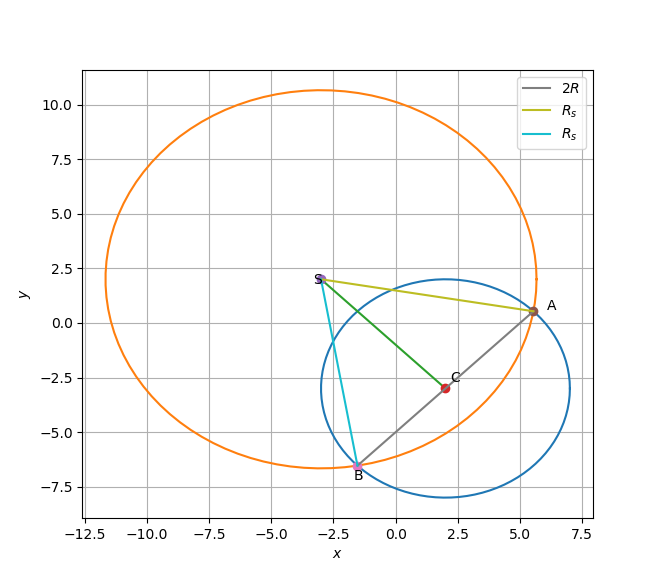
\includegraphics[scale=0.5]{/home/haveesh/Pictures/Figure_5.png}
\end{frame}

\begin{frame}

  
    
    
      \begin{center}

        \font\endfont = cmss10 at 25.40mm
        \color{black}
        \endfont 
        \baselineskip 20.0mm

        The End

      \end{center}    

    
  

\end{frame}


\end{document}